\section{Theorie}
\label{sec:Theorie}



\subsection{Mikrowellen}

Mikrowellen sind elektromagnetische Wellen mit einer Wellenlänge von ca. $\SI{30}{\centi\m}$ bis $\SI{0.3}{\milli\m}$. Da aber die Wirkung der Strahlungseffekte innerhalb eines Schaltungs-Systems von dem Verhältnis zwischen der Größenordung des Systems und der Wellenlänge der vorkommenden Strahlung abhängt, gilt der Bereich der Mikrowellentechnik für Wellenlängen die sehr viel kleiner als die Abmessungen des Systems sind. Mikrowellen werden vielseitig eingesetzt. Sie dienen z.B. in der Luft- und Schiffahrt der Orientierung und der Detektion von anderen Fahrzeugen. Außerdem kommen sie in der Forschung bei Material- und Plasmauntersuchungen zum Einsatz. 

\subsection{Hohlleiter}


\begin{figure}
    \centering
    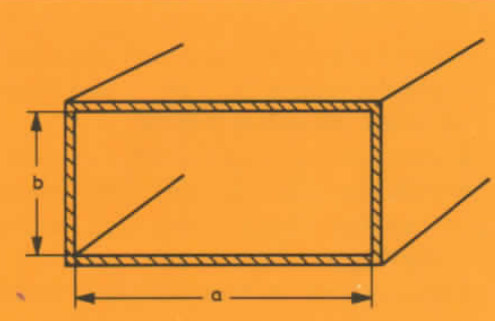
\includegraphics[width=0.5\textwidth]{Bilder/hohlleiter_querschnitt.PNG}
    \caption{Rechteck-Hohlleiter im Querschnitt.\cite{Mikrowellen}}
    \label{fig:hohlleiter}
\end{figure}



Wenn sich elektromagnetische Wellen ungehindert im freien Raum bewegen können, dann breiten sie sich als tranversale, ebene Wellen aus. 
Sobald sie jedoch durch Randbedingungen beschränkt werden, verändern sich die Eigenschaften der Wellen. Diese Randbedigungen können durch einen Hohlleiter realisiert werden. Ein Hohlleiter ist dabei ein Metallrohr mit jeweils unterschiedlicher Querschnittsfläche. In diesem Versuch werden zum leiten der Welle Rechteck-Hohlleiter verwendet, wesswegen im folgenden auch nur auf diese Art von Randbedingungen genauer eingegangen wird. Rechteck-Hohlleiter haben einen konstanten rechteckigen Querschnitt mit jeweils parallelen Wänden. Ein solcher Hohlleiter ist in Abbildung \ref{fig:hohlleiter} dargestellt.
Breitet sich eine Welle in so einem Hohlleiter aus, so wird sie ständig von Wand zu Wand reflektiert. Dabei entstehen theoretisch unedlich viele verschiedene Typen, welche jeweils \textbf{Modus} genannt werden. Aufgrund der Randbedingungen sind die Wellenlänge der freien Welle und die im Hohlleiter unterschiedlich. Der Zusammenhang zwischen der Wellenlänge im freien Raum $\lambda_0$ und der Wellenlänge im Hohlleiter $\lambda_h$ ist über 
\begin{equation}
    \lambda_0 = \frac{1}{\sqrt{\left(\frac{1}{\lambda_h}\right)^2+\left(\frac{1}{2a}\right)^2}}
\end{equation}
gegeben. a beschreibt dabei die Länge der Breitseite des Hohlleiters,
Die Frequenz der Welle lässt sich dann mit $c$ als Lichtgeschwindigkeit im Vakuum über
\begin{equation}
    \label{eqn:f}
    f = \frac{c}{\lambda_0}
\end{equation}
bestimmen.

Die \textbf{Signaldämpfung} wird in $\si{\decibel}$ angegeben und lässt sich aus dem Verhältnis der Leistung ohne vorhandenen Dämpfer $P_1$ und der durch den Dämpfer abgeschwächten Leistung $P_2$ bestimmen.
Die Umrechnung kann über
\begin{equation}
    \left(\frac{P_1}{P_2}\right)_{\si{\decibel}} = 10 \log\frac{P_1}{P_2}
\end{equation}

\subsection{Reflex-Klystron}


\begin{figure}
    \centering
    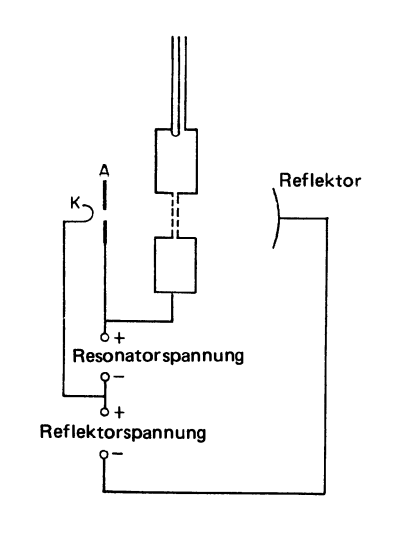
\includegraphics[width=0.5\textwidth]{Bilder/reflex_klystron.PNG}
    \caption{Darstellung eines Reflex-Klystrons.\cite{Mikrowellen}}
    \label{fig:klystron}
\end{figure}

Ein Klystron ist ein Gerät zum erzeugen bzw. verstärken von Mikrowellen. In Abbildung \ref{fig:klystron} ist ein Reflex-Klystron dargestellt. In dem Hohlraumresonator befindet sich ein Wechselfeld. Der kontinuierliche Elektronenstrahl verlässt die Kathode und erfährt beim ersten durchtreten des Gitters des Mikrowellenresonators eine Geschwindigkeitsmodulation. Diese Elektronen werden dann über einen Reflektor reflektiert und passieren erneut das Gitter. Auf diese Weise, wenn die Elektronen-Banches zum richtigen Zeitpunkt das Gitter passieren, werden die Elektronen vom Wechselfeld gebremst, wodurch das Selbige verstärkt wird und Mikrowellen das Klystron verlassen können. Dieser Energieübertrag hat bei Flugzeiten von $t = T(n+\nicefrac{3}{4})$, $n \in $ sein Optimum. $T$ beschreibt die Periodendauer des Wechselfeldes. Über Variation der Reflektorspannung (elektronische Abstimmung) und des Resonatorvolumens (mechanische Abstimmung)
lässt sich die Frequenz und Amplitude des Klystrons verändern. Die Abhängigkeit der Ausgangsleistung von der Reflektorspannung ist in Abbildung \ref{fig:reflektor} dargestellt.

\begin{figure}
    \centering
    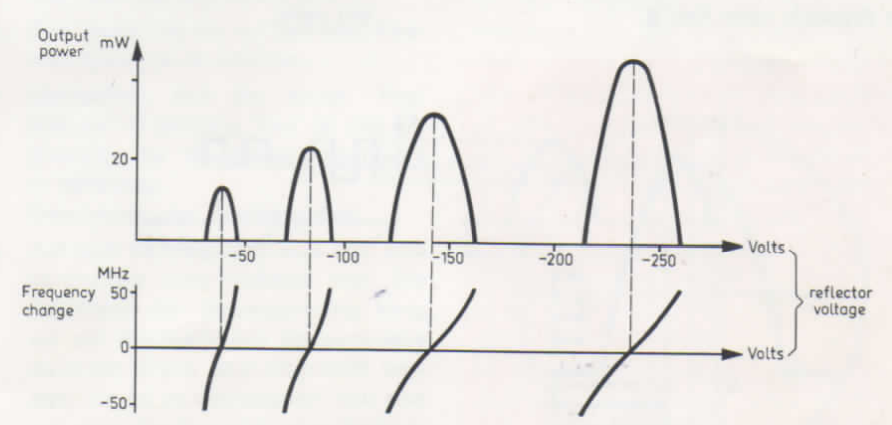
\includegraphics[width=0.8\textwidth]{Bilder/reflektor.PNG}
    \caption{Ausgangsleistung in Abhängigkeit der Reflektorspannung.\cite{Mikrowellen}}
    \label{fig:reflektor}
\end{figure}

\subsection{Stehende Wellen}

Durch Unebenheiten oder gar Grenzflächen kommt es im Hohlleiter zu Reflexionen, bei denen die reflektierten Wellen wieder zurück in Richtung des Generators propagieren. Dadurch setzen sich die resultierenden Wellen aus der Überlagerung von einlaufenden und reflektierten Wellen zusammen. In abgeschlossenen Leitungen endlicher Länge kommt die Umhüllende dieser Überlagerung als \textbf{stehende Welle} vor. Dabei bleibt die Phase der Welle ortsfest. Das "Spannungs-Stehwellen-Verhältnis" (SWR) gibt Aussage über das Verhältnis zwischen maximaler und minimaler Feldstärke auf der Leitung. Es lässt sich also über
\begin{equation}
    S = \frac{E_{\text{max}}}{E_{\text{min}}} = \frac{|E_i|+|E_r|}{|E_i|-|E_r|}
\end{equation}
berechnen. Wobei der Index $r$ für die Feldstärke der reflektierten und $i$ für die der einlaufenden Welle steht.


Im Rahmen des Versuches wird zum Messen des SWR die sogenannte "$3 \si{\decibel}$"- Methode angewandt. Aus den dort gemessen Werten lässt sich das SWR über
\begin{equation}
    \label{eqn:3db}
    S = \sqrt{1+\frac{1}{\sin^2\left(\frac{\pi(d_1-d_2)}{\lambda_h}\right)}}
\end{equation}
bestimmen. 
Über die ebenso verwendete "Abschwächer-Methode" lässt sich das SWR über
\begin{equation}
    \label{eqn:abschw}
    S = 10^{\frac{A_2-A_1}{20}}
\end{equation}
berechnen.
Beide Methoden werden in der Durchführung \ref{sec:Durchführung} näher beschrieben.


\subsection{Einige Bauteile und ihre Funktion}

\begin{figure}
    \label{fig:bauteile}
    \centering
    \subfloat[][Abschluss]{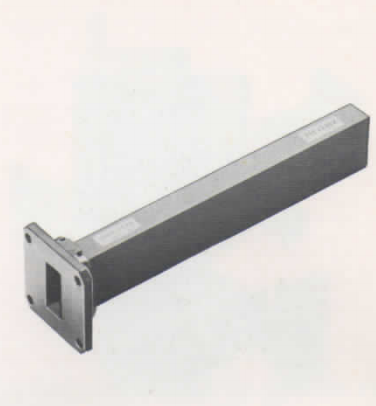
\includegraphics[width=0.3\linewidth]{Bilder/abschluss.PNG}}
    \qquad
    \subfloat[][Dämfungsglied]{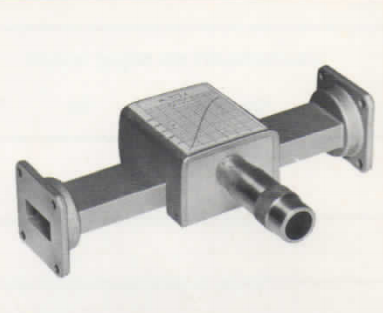
\includegraphics[width=0.4\linewidth]{Bilder/daempfer.PNG}}
    \qquad
    \subfloat[][Gleitschraubentransformator]{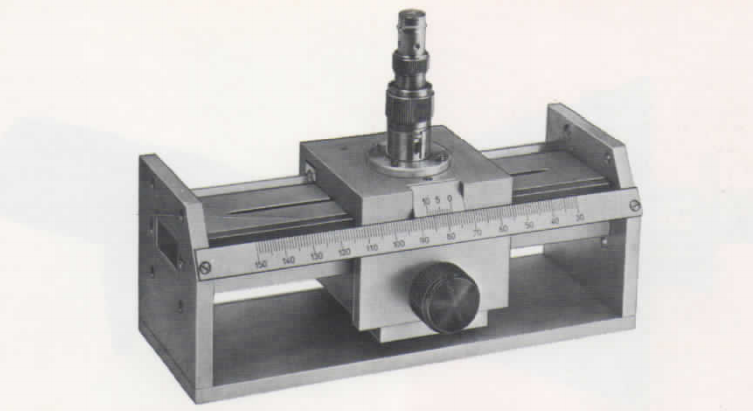
\includegraphics[width=0.5\linewidth]{Bilder/schieber.PNG}}
    \subfloat[][Frequenzmesser]{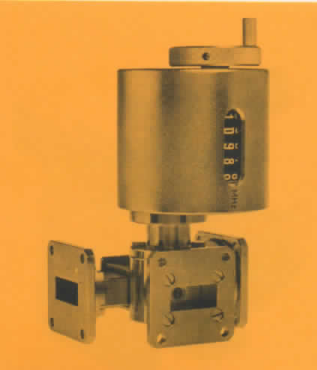
\includegraphics[width=0.3\linewidth]{Bilder/frequenz.PNG}}
    \caption{Einige Bauteile.\cite{Mikrowellen}}
  \end{figure}

Die für den Versuch wichtigsten Bauteile sind neben dem Klystron die in Abbildung \ref{fig:bauteile} dargestellten Komponenten.
Der \textbf{Abschluss} absorbiert, mit Hilfe eines Absorptionsmaterial, beinahe die gesamte Leistung. 
Das \textbf{Dämpfungsglied} dient der Dämpung der Leistung des Feldes. Über eine verschiebare Widerstandsfolie lässt sich die Stärke der Dämpfung einstellen. 
Der \textbf{Gleitschraubentransformator} ist ein Bauteil, welches zum Anpassen eines fehlangepassten Kreises verwendet wird. Die Anpassung wird dabei durch einen variabel verschieb- und senkbaren Sitft realisiert, welcher in der Leitung als beinahe reiner Blindwiderstand wirkt.
Zum Messen der Frequenzen des Systems wird ein \textbf{Frequenzmesser} verwendet. Dieser besteht aus einem Hohlraumresonator mit verstellbarem Volumen. Befindet sich der Frequenzmesser in dem System, so entzieht der Hohlraumresonator die meiste Leistung, wenn die Resonanzfrequenz des Resonators der der im System vorhandenen Frequenz entspricht. So kann also bei maximalem Leistungsentzug auf die Frequenz im System rückgeschlossen werden.








%In knapper Form sind die physikalischen Grundlagen des Versuches, des Messverfahrens, sowie sämtliche für die Auswertung erforderlichen Gleichungen darzustellen. (Keine Herleitung)

%(eventuell die Aufgaben)

%Der Versuchsaufbau: Beschreibung des Versuchs und der Funktionsweise (mit Skizze/Bild/Foto)
